\section{均值与协方差}
\label{sec:rvc-moments}

把两台传感器的读数取平均，波动能减小多少？若两台独立，直觉告诉我们方差减半；可是图~\ref{fig:rvc-sensor-table}的两台读数倾向于一致，平均以后的改善应当少一些。要把“少多少”算出来，需要一个能概括两个量一起偏离中心的数。完整的联合分布在高维时难以列出，这一节用均值向量和协方差矩阵概括它的中心与波动。全节假定所涉及的各分量都有有限二阶矩，即$\mathbb{E}[X_i^{2}]<\infty$；只用到均值的地方，有限一阶矩就够了。

\paragraph{均值向量}
随机向量的中心可以逐个分量描述。设每个分量都有有限期望，定义\term{均值向量}（mean vector）
\begin{equation}
 \bm{\mu}=\mathbb{E}[\bm{X}]=\bigl(\mathbb{E}[X_1],\dots,\mathbb{E}[X_d]\bigr)^{\top}.
 \label{eq:rvc-mean-vector}
\end{equation}
一元时期望是质量分布的重心；这里$\bm{\mu}$是平面或空间中质量分布的重心。传感器表中$\bm{\mu}=(1,1)^{\top}$。三角形模型中，由边缘密度，
\[
 \mathbb{E}[X]=\int_{0}^{1}x\cdot 2x\,\mathrm{d}x=\frac23,\qquad \mathbb{E}[Y]=\int_{0}^{1}y\cdot 2(1-y)\,\mathrm{d}y=\frac13,
\]
$\bm{\mu}=(2/3,1/3)^{\top}$，正是三角形三个顶点坐标的平均，也就是均匀薄板的重心。

期望对随机向量是线性的。在式~\eqref{eq:rvc-joint-expectation}中取$\varphi(x,y)=x+y$，把和或积分拆成两项，得到$\mathbb{E}[X+Y]=\mathbb{E}[X]+\mathbb{E}[Y]$。逐行使用这一点，对$m\times d$常矩阵$\bm{A}$和常向量$\bm{b}\in\mathbb{R}^{m}$，
\begin{equation}
 \mathbb{E}[\bm{A}\bm{X}+\bm{b}]=\bm{A}\bm{\mu}+\bm{b}.
 \label{eq:rvc-mean-affine}
\end{equation}
这里不需要分量之间有任何独立性。矩阵按全书约定用粗体大写字母表示，后面的协方差矩阵$\bm{\Sigma}$也是如此。

\paragraph{协方差与交叉项}
和的均值只依赖各分量的均值，和的方差却不同。记$\mu_X=\mathbb{E}[X]$，$\mu_Y=\mathbb{E}[Y]$，把$X+Y$减去均值后平方展开：
\[
 \operatorname{Var}(X+Y)=\mathbb{E}\Bigl[\bigl((X-\mu_X)+(Y-\mu_Y)\bigr)^{2}\Bigr].
\]
平方展开成三项，再由期望的线性，
\[
 \operatorname{Var}(X+Y)=\operatorname{Var}(X)+\operatorname{Var}(Y)+2\,\mathbb{E}\bigl[(X-\mu_X)(Y-\mu_Y)\bigr].
\]
前两项只依赖边缘分布，最后一项依赖联合分布。这个交叉项就是我们要找的量。

\begin{definition}[协方差]
\label{def:rvc-covariance}
设$\mathbb{E}[X^{2}]<\infty$，$\mathbb{E}[Y^{2}]<\infty$。称
\begin{equation}
 \operatorname{Cov}(X,Y)=\mathbb{E}\bigl[(X-\mu_X)(Y-\mu_Y)\bigr]
 \label{eq:rvc-covariance}
\end{equation}
为$X$与$Y$的\term{协方差}（covariance）。
\end{definition}

有限二阶矩保证这个期望存在：由$\lvert uv\rvert\leq(u^{2}+v^{2})/2$，中心化乘积的绝对值被两个平方项之和控制。展开乘积并用线性，得到常用的计算公式
\begin{equation}
 \operatorname{Cov}(X,Y)=\mathbb{E}[XY]-\mu_X\mu_Y .
 \label{eq:rvc-covariance-formula}
\end{equation}

中心化乘积$(X-\mu_X)(Y-\mu_Y)$的符号有直观意义。以均值点$(\mu_X,\mu_Y)$为原点把平面分成四个象限：两个量同时偏高或同时偏低时，乘积为正；一高一低时，乘积为负。协方差把每个取值对的乘积按质量加权求和。为正，说明“同向偏离”的质量占优；为负，说明“反向偏离”占优。

图~\ref{fig:rvc-cov-quadrants}把传感器表的九个格子画成圆，并标出每格对协方差的贡献$(x-1)(y-1)p_{X,Y}(x,y)$。位于均值线上的格子贡献为零；四个角中，左下与右上各贡献$+0.20$，另两角的概率为零。于是
\[
 \operatorname{Cov}(X,Y)=0.20+0.20=0.40 .
\]
用式~\eqref{eq:rvc-covariance-formula}核对：$XY$只在$x,y\geq1$的四格非零，
\[
 \mathbb{E}[XY]=1\cdot0.20+2\cdot0.10+2\cdot0.10+4\cdot0.20=1.4,
\]
\[
 \operatorname{Cov}(X,Y)=1.4-1\cdot1=0.4 .
\]

\begin{BookInlineFigure}
  \centering
  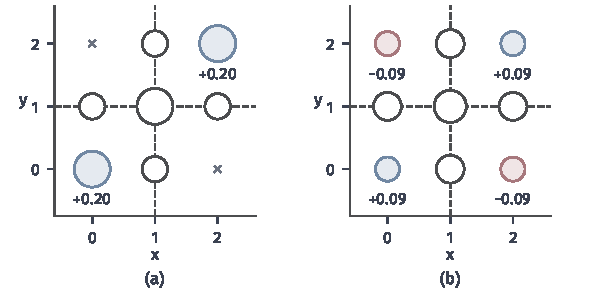
\includegraphics[width=100mm]{figures/07-probability/01-elementary-probability/matplotlib/rvc-cov-quadrants/figure.pdf}
  \caption{协方差是中心化乘积的加权和。圆的面积正比于格子的概率，虚线过均值$(1,1)$。蓝色格子的贡献$(x-1)(y-1)p_{X,Y}(x,y)$为正，红色为负，白色为零，叉号表示概率为零的格子；数字是各格的贡献。(a)传感器表，协方差$0.40$。(b)边缘相同的乘积表，正负贡献抵消，协方差为$0$。}
  \label{fig:rvc-cov-quadrants}
\end{BookInlineFigure}

协方差关于每个变量都是线性的，并且不受平移影响。由定义直接得到：对常数$a,b,c,e$，
\[
 \operatorname{Cov}(aX+b,\,cY+e)=ac\operatorname{Cov}(X,Y),\qquad \operatorname{Cov}(X,X)=\operatorname{Var}(X),
\]
并且对第三个二阶矩有限的变量$X_2$，
\[
 \operatorname{Cov}(X+X_2,\,Y)=\operatorname{Cov}(X,Y)+\operatorname{Cov}(X_2,Y).
\]把这些性质用于$\sum_i a_iX_i$与它自己，就得到有限和的方差展开：
\begin{equation}
 \operatorname{Var}\Bigl(\sum_{i=1}^{n}a_iX_i\Bigr)=\sum_{i=1}^{n}a_i^{2}\operatorname{Var}(X_i)+2\sum_{i<j}a_ia_j\operatorname{Cov}(X_i,X_j).
 \label{eq:rvc-variance-sum}
\end{equation}
$n$个对角项来自各分量自身的波动，$n(n-1)/2$个交叉项来自两两之间的共同波动。

用传感器表算一算。由式~\eqref{eq:rvc-variance-sum}，
\[
 \operatorname{Var}(X+Y)=0.6+0.6+2\cdot0.4=2.0 .
\]
直接核对：把表中格子按$x+y$的值分组，$X+Y$在$\{0,1,2,3,4\}$上各取概率$0.2$，均值为$2$，方差为$(4+1+0+1+4)\times0.2=2$。两台读数的平均$(X+Y)/2$方差为$2.0/4=0.5$，只比单台的$0.6$小一点；若换成图~\ref{fig:rvc-same-marginals}(b)那样独立的两台，交叉项为零，平均的方差是$1.2/4=0.3$，正好减半。

交叉项的符号随系数而变。两台读数之差的方差是
\[
 \operatorname{Var}(X-Y)=0.6+0.6-2\cdot0.4=0.4 .
\]
直接核对：$X-Y$以概率$0.6$取$0$，以概率$0.2$各取$\pm1$，方差为$0.4$。正相关使和的波动变大、差的波动变小，所以比较两台读数之差，比单看一台更容易发现某台失灵：正常时差几乎总在$0$附近。

\paragraph{协方差矩阵}
$d$个分量两两之间都有协方差，排成矩阵便于统一计算。定义\term{协方差矩阵}（covariance matrix）
\begin{equation}
 \bm{\Sigma}=\operatorname{Cov}(\bm{X})=\mathbb{E}\bigl[(\bm{X}-\bm{\mu})(\bm{X}-\bm{\mu})^{\top}\bigr],\qquad
 \bm{\Sigma}_{i,j}=\operatorname{Cov}(X_i,X_j),
 \label{eq:rvc-covariance-matrix}
\end{equation}
其中矩阵的期望逐个元素计算。对角元是各分量的方差，非对角元是协方差。传感器表和三角形模型的协方差矩阵分别是
\[
 \begin{bmatrix}0.6&0.4\\0.4&0.6\end{bmatrix},\qquad
 \begin{bmatrix}1/18&1/36\\1/36&1/18\end{bmatrix}.
\]
后者由边缘密度算出$\mathbb{E}[X^{2}]=1/2$、$\mathbb{E}[Y^{2}]=1/6$，再用上一节的$\mathbb{E}[XY]=1/4$：
\[
 \operatorname{Var}(X)=\tfrac12-\tfrac49=\tfrac1{18},\quad
 \operatorname{Var}(Y)=\tfrac16-\tfrac19=\tfrac1{18},\quad
 \operatorname{Cov}(X,Y)=\tfrac14-\tfrac29=\tfrac1{36}.
\]

式~\eqref{eq:rvc-variance-sum}写成矩阵形式，就是协方差矩阵最重要的性质。

\begin{theorem}[协方差矩阵的性质]
\label{thm:rvc-covariance-matrix}
设$\bm{X}$的各分量有有限二阶矩，协方差矩阵为$\bm{\Sigma}$。对常向量$\bm{a},\bm{b}\in\mathbb{R}^{d}$，
\begin{equation}
 \operatorname{Cov}(\bm{a}^{\top}\bm{X},\,\bm{b}^{\top}\bm{X})=\bm{a}^{\top}\bm{\Sigma}\bm{b},\qquad
 \operatorname{Var}(\bm{a}^{\top}\bm{X})=\bm{a}^{\top}\bm{\Sigma}\bm{a}\geq 0 .
 \label{eq:rvc-quadratic-form}
\end{equation}
因此$\bm{\Sigma}$对称半正定。对$m\times d$常矩阵$\bm{A}$和常向量$\bm{b}\in\mathbb{R}^{m}$，
\begin{equation}
 \operatorname{Cov}(\bm{A}\bm{X}+\bm{b})=\bm{A}\bm{\Sigma}\bm{A}^{\top}.
 \label{eq:rvc-covariance-affine}
\end{equation}
\end{theorem}

\begin{proof}
协方差的定义关于两个变量对称，所以$\bm{\Sigma}$对称。由式~\eqref{eq:rvc-mean-affine}，$\bm{a}^{\top}\bm{X}$的均值是$\bm{a}^{\top}\bm{\mu}$，所以它的中心化是$\bm{a}^{\top}(\bm{X}-\bm{\mu})$；$\bm{b}^{\top}\bm{X}$同理。两个标量之积可以写成
\[
 \bigl(\bm{a}^{\top}(\bm{X}-\bm{\mu})\bigr)\bigl(\bm{b}^{\top}(\bm{X}-\bm{\mu})\bigr)
 =\bm{a}^{\top}(\bm{X}-\bm{\mu})(\bm{X}-\bm{\mu})^{\top}\bm{b}.
\]
右边是矩阵元素的线性组合，取期望时可以逐项进行，得到$\bm{a}^{\top}\bm{\Sigma}\bm{b}$。取$\bm{b}=\bm{a}$，左边是方差，必不小于零，这对一切$\bm{a}$成立，所以$\bm{\Sigma}$半正定。最后，$\bm{A}\bm{X}+\bm{b}$的第$i$个分量是$\bm{A}_{i,:}\bm{X}+b_i$，常数不影响协方差，由第一式，它与第$j$个分量的协方差为$\bm{A}_{i,:}\bm{\Sigma}\bm{A}_{j,:}^{\top}$，这正是$\bm{A}\bm{\Sigma}\bm{A}^{\top}$的$(i,j)$元。
\end{proof}

用式~\eqref{eq:rvc-covariance-affine}可以一次算出几个线性组合的全部方差与协方差。对传感器读数取平均$Z=(X+Y)/2$与差$W=X-Y$，即
\[
 \begin{bmatrix}Z\\W\end{bmatrix}=\bm{A}\begin{bmatrix}X\\Y\end{bmatrix},\qquad
 \bm{A}=\begin{bmatrix}1/2&1/2\\1&-1\end{bmatrix}.
\]
矩阵相乘得到
\[
 \bm{A}\bm{\Sigma}\bm{A}^{\top}
 =\begin{bmatrix}1/2&1/2\\1&-1\end{bmatrix}\begin{bmatrix}0.6&0.4\\0.4&0.6\end{bmatrix}\begin{bmatrix}1/2&1\\1/2&-1\end{bmatrix}
 =\begin{bmatrix}0.5&0\\0&0.4\end{bmatrix}.
\]
对角元与前面分别算出的$0.5$、$0.4$一致；非对角元为零，说明平均与差不相关。原因是两台读数方差相等：由协方差的双线性，交叉的两项互相抵消，
\[
 \operatorname{Cov}(Z,W)=\tfrac12\bigl(\operatorname{Var}(X)-\operatorname{Var}(Y)\bigr)=0 .
\]不相关并不等于独立，例如$W=\pm1$时$Z$只能取$1/2$或$3/2$，而$W=0$时$Z$可以取$0,1,2$。

式~\eqref{eq:rvc-quadratic-form}给协方差矩阵一个几何解释。取单位向量$\bm{a}$，$\bm{a}^{\top}(\bm{X}-\bm{\mu})$是点$\bm{X}$在方向$\bm{a}$上相对重心的有向距离，所以$\bm{a}^{\top}\bm{\Sigma}\bm{a}$是质量沿方向$\bm{a}$的散开程度。把概率看作质量，这正是力学中薄板绕“过重心且垂直于$\bm{a}$的直线”的转动惯量；一元方差是它的一维特例。

$\bm{\Sigma}$是实对称矩阵，可以正交对角化，单位特征向量给出散开程度最大和最小的方向，对应的特征值就是沿这些方向的方差，可参考\BookChapterRef{chap:eigen-spectral-decomposition}{卷二第6章“谱分解”}。三角形模型中，取$\bm{a}=(\cos\varphi,\sin\varphi)^{\top}$，
\[
 v(\varphi)=\bm{a}^{\top}\bm{\Sigma}\bm{a}=\frac{1}{18}+\frac{\sin 2\varphi}{36}.
\]
$\varphi=\pi/4$时取最大值$1/12$，方向$(1,1)^{\top}/\sqrt2$；$\varphi=3\pi/4$时取最小值$1/36$，方向$(1,-1)^{\top}/\sqrt2$。两者正是$\bm{\Sigma}$的两个特征值和特征向量，见图~\ref{fig:rvc-cov-ellipse}。

\begin{BookInlineFigure}
  \centering
  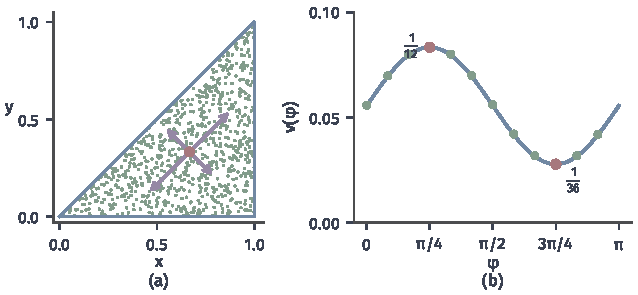
\includegraphics[width=108mm]{figures/07-probability/01-elementary-probability/matplotlib/rvc-cov-ellipse/figure.pdf}
  \caption{协方差矩阵与散开方向。(a)三角形模型的$800$个模拟点（绿，种子$1$），红点为均值$(2/3,1/3)$，紫色双箭头沿两个特征向量，半长等于该方向的标准差$\sqrt{1/12}$与$\sqrt{1/36}$。(b)方向$(\cos\varphi,\sin\varphi)$上的方差$v(\varphi)$（蓝线），红点为最大值与最小值，绿点是同一批模拟点投影后的样本方差。}
  \label{fig:rvc-cov-ellipse}
\end{BookInlineFigure}

半正定而不正定时，存在非零$\bm{a}$使$\bm{a}^{\top}\bm{\Sigma}\bm{a}=0$。这时$\bm{a}^{\top}\bm{X}$的方差为零，由第~\ref{chap:tail-probabilities}章的Chebyshev不等式，对每个$\varepsilon>0$，
\[
 \mathbb{P}\bigl(\lvert\bm{a}^{\top}\bm{X}-\bm{a}^{\top}\bm{\mu}\rvert\geq\varepsilon\bigr)\leq\frac{0}{\varepsilon^{2}}=0 .
\]
也就是说，$\bm{X}$偏离超平面$\bm{a}^{\top}\bm{x}=\bm{a}^{\top}\bm{\mu}$任何正距离的概率都是零，质量全部压在这个超平面上。例如把传感器读数排成$\bm{X}=(X,Y,X+Y)^{\top}$，由式~\eqref{eq:rvc-covariance-affine}，
\[
 \bm{\Sigma}=\begin{bmatrix}0.6&0.4&1.0\\0.4&0.6&1.0\\1.0&1.0&2.0\end{bmatrix},\qquad
 \bm{\Sigma}\begin{bmatrix}1\\1\\-1\end{bmatrix}=\bm{0}.
\]
零特征值对应的方向$(1,1,-1)^{\top}$正好表达了第三个分量等于前两个之和。这种由线性约束造成的奇异协方差，在第~\ref{chap:multivariate-distributions}章的计数向量中还会遇到。

\paragraph{相关系数}
协方差的数值依赖单位：把温度从摄氏度换成另一种刻度，乘以常数$c$，协方差也乘以$c$，而两台传感器之间的联系并没有改变。除以两个标准差，就得到与单位无关的量。

\begin{definition}[相关系数]
\label{def:rvc-correlation}
设$0<\operatorname{Var}(X)<\infty$，$0<\operatorname{Var}(Y)<\infty$，记$\sigma_X,\sigma_Y$为标准差。称
\begin{equation}
 \rho_{X,Y}=\frac{\operatorname{Cov}(X,Y)}{\sigma_X\sigma_Y}
 \label{eq:rvc-correlation}
\end{equation}
为$X$与$Y$的\term{相关系数}（correlation coefficient），不致混淆时简写为$\rho$。
\end{definition}

\begin{theorem}[相关系数的范围]
\label{thm:rvc-correlation-bound}
在上述条件下$-1\leq\rho_{X,Y}\leq 1$。若$\rho_{X,Y}=\pm1$，记
\begin{equation}
 L=\mu_Y+\rho_{X,Y}\frac{\sigma_Y}{\sigma_X}(X-\mu_X),
 \label{eq:rvc-correlation-line}
\end{equation}
则对每个$\varepsilon>0$有$\mathbb{P}(\lvert Y-L\rvert\geq\varepsilon)=0$。反过来，若$Y=a+bX$，$b\neq0$，则$\rho_{X,Y}$等于$b$的符号。
\end{theorem}

\begin{proof}
把两个变量标准化，令$U=(X-\mu_X)/\sigma_X$，$V=(Y-\mu_Y)/\sigma_Y$，则
\[
 \mathbb{E}[U^{2}]=\mathbb{E}[V^{2}]=1,\qquad \mathbb{E}[UV]=\rho .
\]
考虑非负随机变量$(V-\rho U)^{2}$，展开后取期望：
\[
 0\leq\mathbb{E}\bigl[(V-\rho U)^{2}\bigr]=\mathbb{E}[V^{2}]-2\rho\,\mathbb{E}[UV]+\rho^{2}\mathbb{E}[U^{2}]=1-\rho^{2},
\]
所以$\rho^{2}\leq1$。

若$\rho^{2}=1$，上式说明$\mathbb{E}[(V-\rho U)^{2}]=0$。对每个$\delta>0$，由第~\ref{chap:tail-probabilities}章的Markov不等式，
\[
 \mathbb{P}\bigl(\lvert V-\rho U\rvert\geq\delta\bigr)=\mathbb{P}\bigl((V-\rho U)^{2}\geq\delta^{2}\bigr)\leq\frac{0}{\delta^{2}}=0 .
\]
由式~\eqref{eq:rvc-correlation-line}，$\sigma_Y(V-\rho U)=Y-L$，取$\delta=\varepsilon/\sigma_Y$即得结论。

反过来，若$Y=a+bX$，则$\operatorname{Cov}(X,Y)=b\sigma_X^{2}$，$\sigma_Y=\lvert b\rvert\sigma_X$，代入式~\eqref{eq:rvc-correlation}得$\rho=b/\lvert b\rvert$。
\end{proof}

这个证明与内积空间中的Cauchy--Schwarz不等式是同一个论证：把$\mathbb{E}[UV]$看作两个中心化变量的内积，相关系数就是它们夹角的余弦，可参考\BookChapterRef{chap:inner-product-spaces}{卷二第4章“内积空间”}。定理的第二部分只说$Y$偏离直线$L$任何正距离的概率为零；第~\ref{chap:probability-spaces}章会说明这等价于$\mathbb{P}(Y=L)=1$。

两个贯穿例子的相关系数是
\[
 \rho_{\text{传感器}}=\frac{0.4}{\sqrt{0.6\cdot0.6}}=\frac23,\qquad
 \rho_{\text{三角形}}=\frac{1/36}{\sqrt{(1/18)(1/18)}}=\frac12 .
\]
对图~\ref{fig:rvc-fgm}的密度族，两个边缘的均值都是$1/2$，密度中的常数项$1$对应独立部分，贡献的协方差为零，于是
\[
 \operatorname{Cov}(X,Y)=\theta\Bigl(\int_{0}^{1}x(1-2x)\,\mathrm{d}x\Bigr)^{2}=\theta\Bigl(-\frac16\Bigr)^{2}=\frac{\theta}{36}.
\]
边缘方差为$1/12$，所以$\rho=\theta/3$，绝对值不超过$1/3$：这个族只能表达较弱的联系。

相关系数衡量的是散点向一条直线集中的程度，而不是直线的斜率。图~\ref{fig:rvc-correlation}前三幅中，$\rho=0.9$的点紧贴上升直线，$\rho=-0.6$的点较松散地沿下降方向分布，$\rho=0$的点看不出线性趋势。第四幅中$Y$几乎由$X$决定，相关系数却为零：抛物线左右两支对“同向”和“反向”的贡献互相抵消。

\begin{BookInlineFigure}
  \centering
  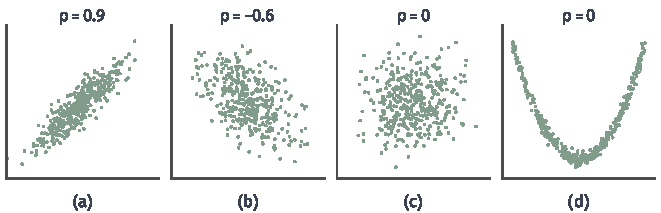
\includegraphics[width=112mm]{figures/07-probability/01-elementary-probability/matplotlib/rvc-correlation/figure.pdf}
  \caption{不同相关系数下的散点，每幅$400$个模拟点（种子$7$）。(a)至(c)中$X,Y$都服从$\mathcal{N}(0,1)$，取$Y=\rho X+\sqrt{1-\rho^{2}}\,Z$，$Z\sim\mathcal{N}(0,1)$与$X$独立，相关系数分别为$0.9$、$-0.6$、$0$。(d)中$X\sim\operatorname{Unif}(-\sqrt3,\sqrt3)$，$Y=X^{2}-1+0.1Z$，相关系数为$0$。}
  \label{fig:rvc-correlation}
\end{BookInlineFigure}

“集中于直线的程度”可以精确表述。用直线$a+bX$近似$Y$，以均方误差$\mathbb{E}[(Y-a-bX)^{2}]$衡量好坏。对固定的$b$，记$W=Y-bX$。把$W-a$拆成$(W-\mathbb{E}[W])+(\mathbb{E}[W]-a)$，交叉项的期望为零，于是
\[
 \mathbb{E}\bigl[(W-a)^{2}\bigr]=\operatorname{Var}(W)+\bigl(\mathbb{E}[W]-a\bigr)^{2}.
\]
最好的$a$是$\mathbb{E}[W]$，剩下的误差是
\[
 \operatorname{Var}(Y-bX)=\operatorname{Var}(Y)-2b\operatorname{Cov}(X,Y)+b^{2}\operatorname{Var}(X).
\]
这是$b$的二次函数，对$b$求导并令导数为零，最小点是
\[
 b^{*}=\frac{\operatorname{Cov}(X,Y)}{\operatorname{Var}(X)}.
\]
代回得到最小均方误差
\begin{equation}
 \min_{a,b}\mathbb{E}\bigl[(Y-a-bX)^{2}\bigr]=\operatorname{Var}(Y)\,(1-\rho_{X,Y}^{2}).
 \label{eq:rvc-best-line}
\end{equation}
所以$\rho^{2}$是最佳直线能解释的那一部分方差。$\rho=0$时最佳斜率为零，直线对预测$Y$毫无帮助；但这只说明直线无用，曲线仍可能很有用，图~\ref{fig:rvc-correlation}(d)就是这样。

\paragraph{平均能把波动降低多少}
现在回答本节开头的问题。设$n$台传感器的读数$X_1,\dots,X_n$方差都是$\sigma^{2}$，任意两台的相关系数都是$\rho$，即协方差都是$\rho\sigma^{2}$。由式~\eqref{eq:rvc-variance-sum}，取$a_i=1/n$，对角项共$n$个，交叉项共$n(n-1)/2$个，
\[
 \operatorname{Var}(\bar{X}_n)=\frac{1}{n^{2}}\Bigl(n\sigma^{2}+n(n-1)\rho\sigma^{2}\Bigr),
\]
其中$\bar{X}_n=(X_1+\dots+X_n)/n$。整理得
\begin{equation}
 \operatorname{Var}(\bar{X}_n)=\sigma^{2}\Bigl(\frac1n+\Bigl(1-\frac1n\Bigr)\rho\Bigr).
 \label{eq:rvc-equicorrelated-average}
\end{equation}

两台传感器的情形，$n=2$，$\sigma^{2}=0.6$，$\rho=2/3$，代入得$0.6\times(1/2+1/3)=0.5$，与前面直接计算的结果一致。$\rho=0$时上式变成$\sigma^{2}/n$，平均$n$次把方差降为$1/n$。$\rho>0$时，$n\to\infty$，方差趋于$\rho\sigma^{2}$而不是零：各台共有的那部分波动，例如同一股气流同时影响所有传感器，无论平均多少台都消不掉。

\begin{BookInlineFigure}
  \centering
  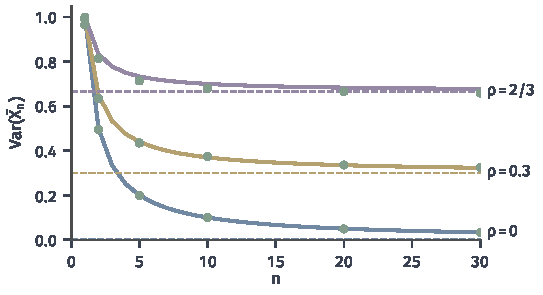
\includegraphics[width=92mm]{figures/07-probability/01-elementary-probability/matplotlib/rvc-average-variance/figure.pdf}
  \caption{$n$个方差为$1$、两两相关系数为$\rho$的读数，其平均的方差。实线是式~\eqref{eq:rvc-equicorrelated-average}，蓝、黄、紫分别对应$\rho=0,0.3,2/3$；虚线是极限$\rho$。绿点是$4000$次模拟的样本方差（种子$11$），每次取$X_i=\sqrt{\rho}\,Z_0+\sqrt{1-\rho}\,Z_i$，$Z_0,Z_1,\dots$相互独立且服从$\mathcal{N}(0,1)$。}
  \label{fig:rvc-average-variance}
\end{BookInlineFigure}

图~\ref{fig:rvc-average-variance}中，模拟用的构造$X_i=\sqrt{\rho}\,Z_0+\sqrt{1-\rho}\,Z_i$把每个读数拆成共同部分$Z_0$和各自部分$Z_i$。平均时各自部分的方差按$1/n$缩小，共同部分原样保留，这正是式~\eqref{eq:rvc-equicorrelated-average}两项的来源。

\paragraph{相关与独立}
协方差为零的两个变量称为\term{不相关}（uncorrelated）。独立变量一定不相关：若$X,Y$独立且二阶矩有限，在定理~\ref{thm:rvc-product-expectation}中取$g(x)=x-\mu_X$，$h(y)=y-\mu_Y$，得到
\[
 \operatorname{Cov}(X,Y)=\mathbb{E}[X-\mu_X]\,\mathbb{E}[Y-\mu_Y]=0 .
\]
因此两两独立的变量之和，方差等于方差之和；式~\eqref{eq:rvc-variance-sum}只需要交叉项为零，也就是只需要两两不相关。

反过来不成立，因为协方差只检查一种特定的乘积。令$X$等可能取$-1,0,1$，$Y=X^{2}$。则$\mathbb{E}[X]=0$，$\mathbb{E}[XY]=\mathbb{E}[X^{3}]=0$，所以$\operatorname{Cov}(X,Y)=0$。可是$Y$完全由$X$决定，独立性不成立：
\[
 \mathbb{P}(X=0,\,Y=1)=0\neq\mathbb{P}(X=0)\,\mathbb{P}(Y=1)=\tfrac13\cdot\tfrac23 .
\]

连续的例子是单位圆盘上的均匀分布，密度在圆盘内为$1/\pi$。把$(x,y)$换成$(-x,y)$，密度不变而$xy$变号，所以$\mathbb{E}[XY]=-\mathbb{E}[XY]=0$；同理$\mathbb{E}[X]=0$，协方差为零。圆盘不是乘积形区域，按上一节的判别，两个分量不独立。具体地，$\mathbb{P}(X>0.9)$与$\mathbb{P}(Y>0.5)$都为正，而点$(x,y)$满足$x>0.9$、$y>0.5$时$x^{2}+y^{2}>0.81+0.25>1$，落在圆盘外，所以$\mathbb{P}(X>0.9,\,Y>0.5)=0$。

\begin{BookInlineFigure}
  \centering
  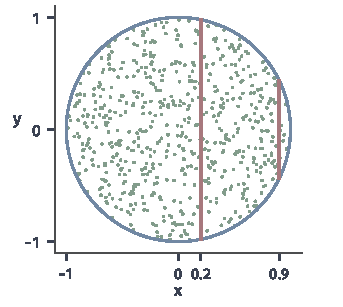
\includegraphics[width=58mm]{figures/07-probability/01-elementary-probability/matplotlib/rvc-disk/figure.pdf}
  \caption{单位圆盘上的均匀分布：不相关但不独立。绿点是$600$个模拟点（种子$3$），样本相关系数约为$-0.01$。红线段是$x=0.2$与$x=0.9$处$y$能取到的范围，分别为$\lvert y\rvert\leq0.98$和$\lvert y\rvert\leq0.44$。}
  \label{fig:rvc-disk}
\end{BookInlineFigure}

图~\ref{fig:rvc-disk}显示了依赖的方式：$X$靠近$\pm1$时，$Y$被挤到$0$附近，$X$靠近$0$时，$Y$可以取到$\pm1$附近。依赖体现在$Y$的散开程度随$X$改变，而不是$Y$的平均位置随$X$线性升降，协方差看不见这种依赖。表~\ref{tab:rvc-dependence}汇总本节的几个关系。

\begin{BookInlineTable}
  \centering
  \caption{独立、不相关与完全线性相关}
  \label{tab:rvc-dependence}
  \begin{tabular}{lll}
    \toprule
    关系 & 要求 & 可以推出 \\
    \midrule
    独立 & 联合分布分解为边缘之积 & 函数仍独立；有矩时不相关 \\
    不相关 & $\operatorname{Cov}(X,Y)=0$ & 和的方差等于方差之和 \\
    $\rho=\pm1$ & 达到相关系数的界 & $Y$偏离某条直线的概率为零 \\
    \bottomrule
  \end{tabular}
\end{BookInlineTable}

表中第一行到第二行只有单向的箭头；零相关只排除线性关联，不排除依赖。在多元高斯模型中，不相关与独立恰好等价，那是第~\ref{chap:multivariate-distributions}章的一个特殊结论，不能推广到一般分布。
